\chapter{In the Beginning...} \label{ch:chapter1}

Quisque facilisis erat a dui. Nam malesuada ornare dolor. Cras gravida, diam sit amet rhoncus ornare, erat elit consectetuer erat, id egestas pede nibh eget odio. Proin tincidunt, velit vel porta elementum, magna diam molestie sapien, non aliquet massa pede eu diam. Aliquam iaculis. Fusce et ipsum et nulla tristique facilisis. Donec eget sem sit amet ligula viverra gravida. Etiam vehicula urna vel turpis. Suspendisse sagittis ante a urna. Morbi a est quis orci consequat rutrum. Nullam egestas feugiat felis. Integer adipiscing semper ligula. Nunc molestie, nisl sit amet cursus convallis, sapien lectus pretium metus, vitae pretium enim wisi id lectus. Donec vestibulum. Etiam vel nibh. Nulla facilisi. Mauris pharetra. Donec augue. Fusce ultrices, neque id dignissim ultrices, tellus mauris dictum elit, vel lacinia enim metus eu nunc.

Proin at eros non eros adipiscing mollis. Donec semper turpis sed diam. Sed consequat ligula nec tortor. Integer eget sem. Ut vitae enim eu est vehicula gravida. Morbi ipsum ipsum, porta nec, tempor id, auctor vitae, purus. Fig.~\ref{fig:1fig3} shows the various types of Pellentesque neque.

\begin{figure}[htb]
\begin{center}
\includegraphics[width=0.75\textwidth]{content/figures/fig3}
\caption{Morbi id urna in diam dignissim feugiat \protect\cite{Eigen1971}}
\label{fig:1fig3}
\end{center}
\end{figure}

Nullam ultrices, diam tempus vulputate egestas, eros pede varius leo, sed imperdiet lectus est ornare odio. Lorem ipsum dolor sit amet, consectetuer adipiscing elit. Proin consectetuer velit in dui. Phasellus wisi purus, interdum vitae, rutrum accumsan, viverra in, velit. Sed enim risus, congue non, tristique in, commodo eu, metus. Aenean tortor mi, imperdiet id, gravida eu, posuere eu, felis \cite{Knuth1968}. Mauris sollicitudin, turpis in hendrerit sodales, lectus ipsum pellentesque ligula, sit amet scelerisque urna nibh ut arcu. Aliquam in lacus. Vestibulum ante ipsum primis in faucibus orci luctus et ultrices posuere cubilia Curae; Nulla placerat aliquam wisi. Mauris viverra odio. Quisque fermentum pulvinar odio. Proin posuere est vitae ligula. Etiam euismod. Cras a eros.

\section{The road ahead}

This chapter defines the conventions used in this content and provides a brief summary of
the basic gas dynamic concepts used. A review of literature provides a brief summary of work
done by various authors and at the Naval Ordinance Laboratory in Maryland in the USA, on the
shock-on-shock problem.

Chapter 2 details the shock tube design, its construction and problems that were encountered
during the commissioning of the tube.

Chapter 3 describes a number of pseudo-steady shock interactions, $\ldots$ of the
shock-on-shock problem.

$\vdots$

\subsection{Closing Thoughts}\label{sec:closingthoughts}

In closing, Chapter 7 reviews the work presented here, drawing conclusions from the results of
the preceding chapters, presenting a new classification of shock-supersonic body interactions
and making recommendations for future work. This last chapter is followed by an appendix
which contains a description of a typical version of the controlling source code of the
numerical model.

\section{Conventions}\label{sec:conventions}

Certain conventions will be applied in this thesis. These are laid out here and are applied to a
number of basic flow equations. Unless otherwise stated, the positive flow direction will be
$\ldots$

It is assumed that the reader is familiar with the techniques for deriving the Rankine-Hugoniot
equations and its two-dimensional variants, so while these equations have been included in the
form used within this text, the derivation has been left to more fundamental texts such as
White \cite{Knuth1968}.

For one-dimensional flow through a stationary shock:

\begin{figure}[htb]
\begin{center}
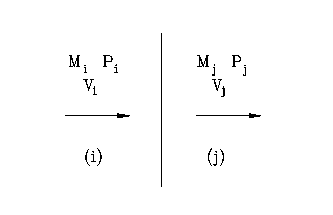
\includegraphics[width=0.6\textwidth]{content/figures/1fig6.eps}
\caption{Flow through a one-dimensional shock.}
\label{fig:1fig6}
\end{center}
\end{figure}

\begin{subequations} \label{eq:r-hn}
\begin{equation}
\left( \frac{a_j}{a_i}\right) ^2=\frac{T_j}{T_i}=\frac{\left( \frac2{\gamma-1}+M_i^2\right)
\left( \frac{2\gamma }{\gamma -1}M_i^2-1\right) }{\left( \frac{\gamma +1}{\gamma -1}
\right) ^2M_i^2}  \label{eq:r-hn1}
\end{equation}

\begin{equation}
\frac{P_j}{P_i}=\frac{\gamma +1}{\gamma -1}\left( \frac{2\gamma }{\gamma -1}M_i^2-1
\right)  \label{eq:r-hn2}
\end{equation}

\begin{equation}
M_j^2=\frac{\left( \frac 2{\gamma -1}+M_i^2\right) }{\left( \frac{2\gamma }{\gamma -1}
M_i^2-1\right) }  \label{eq:r-hn3}
\end{equation}
\end{subequations}

These equations can then be expanded for the two-dimensional case to:

\begin{subequations} \label{eq:r-ho}
\begin{equation}
\frac{P_j}{P_i}=\frac{\gamma -1}{\gamma +1}\left( \frac{2\gamma }{\gamma -1}M_i^2
\sin ^2\phi _j-1\right)  \label{eq:r-ho1}
\end{equation}

\begin{equation}
\left( \frac{a_j}{a_i}\right) ^2=\frac{T_j}{T_i}=\frac{\left( \frac2{\gamma-1}+M_i^2\sin ^2
\phi _j\right) \left( \frac{2\gamma }{\gamma -1}M_i^2\sin ^2\phi _j-1\right) }{\left( 
\frac{\gamma +1}{\gamma -1}\right)^2M_i^2\sin^2\phi _j}  \label{eq:r-ho2}
\end{equation}

\begin{equation}
M_j^2=\frac{\left(M_i^2\sin ^2\phi _j+\frac 2{\gamma-1}\right)^2 + \left(\frac{\gamma +1}
{\gamma -1}\right)^2 M_i^2\sin ^2\phi _j M_i^2\cos ^2\phi _j}{\left( M_i^2\sin ^2\phi _j+
\frac 2{\gamma-1}\right)\left( \frac{2\gamma }{\gamma -1}M_i^2\sin ^2\phi _j-1\right) }
\label{eq:r-ho3}
\end{equation}

\begin{equation}
\tan \theta _j=\cot \phi _j\left( \frac{M_i^2\sin ^2\phi _j-1}{\frac{\gamma+1}2 M_i^2 - 
\left(M_i^2 \sin^2 \phi_j -1 \right)}\right) \label{eq:r-ho4}
\end{equation}
\end{subequations}

Eqn.~\ref{eq:r-ho} is written as used in this work and differs slightly from generally accepted
convention, but is in a form which can readily be rewritten in terms of the density ratio across
the shock ($\Lambda_{ij}$). $\gamma $ is determined by the type of fluid the shock travels in,
usually air. Given any two of $\frac{P_j}{P_i},\frac{T_j}{T_i}, \theta, \phi $ or $M$, all other
fluid properties across the oblique shock can be determined.

$\vdots$ \\

Additional litterature reviewed here \\

$\vdots$

example of a table $\dots$

Table \ref{tab:1table1} gives a number of theoretical maxima for a number of driver/driven gas
combinations:

\begin{table}[htb]
\caption{Limiting Mach numbers for various Driver/Driven gas combinations %
\protect\cite{Knuth1968}} \label{tab:1table1}
\centering
\begin{tabular}{|c|c|c|c|}
\hline
\textbf{Driver/Driven Gas} & $\mathbf{\gamma }_1$ & $\mathbf{\gamma }_2$ & 
\textbf{M}$_{s_\infty }$ \\ \hline
Air/Air & 1.404 & 1.404 & 6.16 \\ \hline
He/Air & 1.667 & 1.404 & 10.6 \\ \hline
He/N$_2$ & 1.667 & 1.407 & 10.4 \\ \hline
He/Ar & 1.667 & 1.667 & 12.7 \\ \hline
H$_2$/Air & 1.407 & 1.404 & 22.5 \\ \hline
H$_2$/N$_2$ & 1.407 & 1.404 & 22.1 \\ \hline
H$_2$/Ar & 1.407 & 1.667 & 26.8 \\ \hline
\end{tabular}
\end{table}

\section{Objectives} \label{sec:1sec7}

A number of clear objectives were identified and pursued for this thesis. These objectives can
be summed up as:
\begin{itemize}
\item  Design and commission a facility for testing two-dimensional shock-on-shock
interactions.
\item  A computational model of the interaction is to be built-up using analytical methods as
described by Smyrl \cite{Knuth1968} and by Li and Ben-Dor \cite{Knuth1968}, with particular focus on
the latter.
\item  A numerical study using an adaptive refinement computational fluid dynamic Euler code
developed at the School of Mechanical Engineering by L. Felthun \cite{Knuth1968}.
\item  An updated set of criteria are to be defined for determining the type of interaction
configuration encountered.
\end{itemize}